
%% bare_conf.tex
%% V1.4b
%% 2015/08/26
%% by Michael Shell
%% See:
%% http://www.michaelshell.org/
%% for current contact information.
%%
%% This is a skeleton file demonstrating the use of IEEEtran.cls
%% (requires IEEEtran.cls version 1.8b or later) with an IEEE
%% conference paper.
%%
%% Support sites:
%% http://www.michaelshell.org/tex/ieeetran/
%% http://www.ctan.org/pkg/ieeetran
%% and
%% http://www.ieee.org/

%%*************************************************************************
%% Legal Notice:
%% This code is offered as-is without any warranty either expressed or
%% implied; without even the implied warranty of MERCHANTABILITY or
%% FITNESS FOR A PARTICULAR PURPOSE! 
%% User assumes all risk.
%% In no event shall the IEEE or any contributor to this code be liable for
%% any damages or losses, including, but not limited to, incidental,
%% consequential, or any other damages, resulting from the use or misuse
%% of any information contained here.
%%
%% All comments are the opinions of their respective authors and are not
%% necessarily endorsed by the IEEE.
%%
%% This work is distributed under the LaTeX Project Public License (LPPL)
%% ( http://www.latex-project.org/ ) version 1.3, and may be freely used,
%% distributed and modified. A copy of the LPPL, version 1.3, is included
%% in the base LaTeX documentation of all distributions of LaTeX released
%% 2003/12/01 or later.
%% Retain all contribution notices and credits.
%% ** Modified files should be clearly indicated as such, including  **
%% ** renaming them and changing author support contact information. **
%%*************************************************************************


% *** Authors should verify (and, if needed, correct) their LaTeX system  ***
% *** with the testflow diagnostic prior to trusting their LaTeX platform ***
% *** with production work. The IEEE's font choices and paper sizes can   ***
% *** trigger bugs that do not appear when using other class files.       ***                          ***
% The testflow support page is at:
% http://www.michaelshell.org/tex/testflow/



\documentclass[conference]{IEEEtran}
% Some Computer Society conferences also require the compsoc mode option,
% but others use the standard conference format.
%
% If IEEEtran.cls has not been installed into the LaTeX system files,
% manually specify the path to it like:
% \documentclass[conference]{../sty/IEEEtran}





% Some very useful LaTeX packages include:
% (uncomment the ones you want to load)


% *** MISC UTILITY PACKAGES ***
%
%\usepackage{ifpdf}
% Heiko Oberdiek's ifpdf.sty is very useful if you need conditional
% compilation based on whether the output is pdf or dvi.
% usage:
% \ifpdf
%   % pdf code
% \else
%   % dvi code
% \fi
% The latest version of ifpdf.sty can be obtained from:
% http://www.ctan.org/pkg/ifpdf
% Also, note that IEEEtran.cls V1.7 and later provides a builtin
% \ifCLASSINFOpdf conditional that works the same way.
% When switching from latex to pdflatex and vice-versa, the compiler may
% have to be run twice to clear warning/error messages.






% *** CITATION PACKAGES ***
%
%\usepackage{cite}
% cite.sty was written by Donald Arseneau
% V1.6 and later of IEEEtran pre-defines the format of the cite.sty package
% \cite{} output to follow that of the IEEE. Loading the cite package will
% result in citation numbers being automatically sorted and properly
% "compressed/ranged". e.g., [1], [9], [2], [7], [5], [6] without using
% cite.sty will become [1], [2], [5]--[7], [9] using cite.sty. cite.sty's
% \cite will automatically add leading space, if needed. Use cite.sty's
% noadjust option (cite.sty V3.8 and later) if you want to turn this off
% such as if a citation ever needs to be enclosed in parenthesis.
% cite.sty is already installed on most LaTeX systems. Be sure and use
% version 5.0 (2009-03-20) and later if using hyperref.sty.
% The latest version can be obtained at:
% http://www.ctan.org/pkg/cite
% The documentation is contained in the cite.sty file itself.






% *** GRAPHICS RELATED PACKAGES ***
%
\ifCLASSINFOpdf
   \usepackage[pdftex]{graphicx}
  % declare the path(s) where your graphic files are
   \graphicspath{{./figs/}}
  % and their extensions so you won't have to specify these with
  % every instance of \includegraphics
   \DeclareGraphicsExtensions{.pdf,.jpeg,.png}
\else
  % or other class option (dvipsone, dvipdf, if not using dvips). graphicx
  % will default to the driver specified in the system graphics.cfg if no
  % driver is specified.
  % \usepackage[dvips]{graphicx}
  % declare the path(s) where your graphic files are
  % \graphicspath{{../eps/}}
  % and their extensions so you won't have to specify these with
  % every instance of \includegraphics
  % \DeclareGraphicsExtensions{.eps}
\fi
% graphicx was written by David Carlisle and Sebastian Rahtz. It is
% required if you want graphics, photos, etc. graphicx.sty is already
% installed on most LaTeX systems. The latest version and documentation
% can be obtained at: 
% http://www.ctan.org/pkg/graphicx
% Another good source of documentation is "Using Imported Graphics in
% LaTeX2e" by Keith Reckdahl which can be found at:
% http://www.ctan.org/pkg/epslatex
%
% latex, and pdflatex in dvi mode, support graphics in encapsulated
% postscript (.eps) format. pdflatex in pdf mode supports graphics
% in .pdf, .jpeg, .png and .mps (metapost) formats. Users should ensure
% that all non-photo figures use a vector format (.eps, .pdf, .mps) and
% not a bitmapped formats (.jpeg, .png). The IEEE frowns on bitmapped formats
% which can result in "jaggedy"/blurry rendering of lines and letters as
% well as large increases in file sizes.
%
% You can find documentation about the pdfTeX application at:
% http://www.tug.org/applications/pdftex





% *** MATH PACKAGES ***
%
%\usepackage{amsmath}
% A popular package from the American Mathematical Society that provides
% many useful and powerful commands for dealing with mathematics.
%
% Note that the amsmath package sets \interdisplaylinepenalty to 10000
% thus preventing page breaks from occurring within multiline equations. Use:
%\interdisplaylinepenalty=2500
% after loading amsmath to restore such page breaks as IEEEtran.cls normally
% does. amsmath.sty is already installed on most LaTeX systems. The latest
% version and documentation can be obtained at:
% http://www.ctan.org/pkg/amsmath





% *** SPECIALIZED LIST PACKAGES ***
%
%\usepackage{algorithmic}
% algorithmic.sty was written by Peter Williams and Rogerio Brito.
% This package provides an algorithmic environment fo describing algorithms.
% You can use the algorithmic environment in-text or within a figure
% environment to provide for a floating algorithm. Do NOT use the algorithm
% floating environment provided by algorithm.sty (by the same authors) or
% algorithm2e.sty (by Christophe Fiorio) as the IEEE does not use dedicated
% algorithm float types and packages that provide these will not provide
% correct IEEE style captions. The latest version and documentation of
% algorithmic.sty can be obtained at:
% http://www.ctan.org/pkg/algorithms
% Also of interest may be the (relatively newer and more customizable)
% algorithmicx.sty package by Szasz Janos:
% http://www.ctan.org/pkg/algorithmicx




% *** ALIGNMENT PACKAGES ***
%
%\usepackage{array}
% Frank Mittelbach's and David Carlisle's array.sty patches and improves
% the standard LaTeX2e array and tabular environments to provide better
% appearance and additional user controls. As the default LaTeX2e table
% generation code is lacking to the point of almost being broken with
% respect to the quality of the end results, all users are strongly
% advised to use an enhanced (at the very least that provided by array.sty)
% set of table tools. array.sty is already installed on most systems. The
% latest version and documentation can be obtained at:
% http://www.ctan.org/pkg/array


% IEEEtran contains the IEEEeqnarray family of commands that can be used to
% generate multiline equations as well as matrices, tables, etc., of high
% quality.




% *** SUBFIGURE PACKAGES ***
%\ifCLASSOPTIONcompsoc
%  \usepackage[caption=false,font=normalsize,labelfont=sf,textfont=sf]{subfig}
%\else
%  \usepackage[caption=false,font=footnotesize]{subfig}
%\fi
% subfig.sty, written by Steven Douglas Cochran, is the modern replacement
% for subfigure.sty, the latter of which is no longer maintained and is
% incompatible with some LaTeX packages including fixltx2e. However,
% subfig.sty requires and automatically loads Axel Sommerfeldt's caption.sty
% which will override IEEEtran.cls' handling of captions and this will result
% in non-IEEE style figure/table captions. To prevent this problem, be sure
% and invoke subfig.sty's "caption=false" package option (available since
% subfig.sty version 1.3, 2005/06/28) as this is will preserve IEEEtran.cls
% handling of captions.
% Note that the Computer Society format requires a larger sans serif font
% than the serif footnote size font used in traditional IEEE formatting
% and thus the need to invoke different subfig.sty package options depending
% on whether compsoc mode has been enabled.
%
% The latest version and documentation of subfig.sty can be obtained at:
% http://www.ctan.org/pkg/subfig




% *** FLOAT PACKAGES ***
%
%\usepackage{fixltx2e}
% fixltx2e, the successor to the earlier fix2col.sty, was written by
% Frank Mittelbach and David Carlisle. This package corrects a few problems
% in the LaTeX2e kernel, the most notable of which is that in current
% LaTeX2e releases, the ordering of single and double column floats is not
% guaranteed to be preserved. Thus, an unpatched LaTeX2e can allow a
% single column figure to be placed prior to an earlier double column
% figure.
% Be aware that LaTeX2e kernels dated 2015 and later have fixltx2e.sty's
% corrections already built into the system in which case a warning will
% be issued if an attempt is made to load fixltx2e.sty as it is no longer
% needed.
% The latest version and documentation can be found at:
% http://www.ctan.org/pkg/fixltx2e


%\usepackage{stfloats}
% stfloats.sty was written by Sigitas Tolusis. This package gives LaTeX2e
% the ability to do double column floats at the bottom of the page as well
% as the top. (e.g., "\begin{figure*}[!b]" is not normally possible in
% LaTeX2e). It also provides a command:
%\fnbelowfloat
% to enable the placement of footnotes below bottom floats (the standard
% LaTeX2e kernel puts them above bottom floats). This is an invasive package
% which rewrites many portions of the LaTeX2e float routines. It may not work
% with other packages that modify the LaTeX2e float routines. The latest
% version and documentation can be obtained at:
% http://www.ctan.org/pkg/stfloats
% Do not use the stfloats baselinefloat ability as the IEEE does not allow
% \baselineskip to stretch. Authors submitting work to the IEEE should note
% that the IEEE rarely uses double column equations and that authors should try
% to avoid such use. Do not be tempted to use the cuted.sty or midfloat.sty
% packages (also by Sigitas Tolusis) as the IEEE does not format its papers in
% such ways.
% Do not attempt to use stfloats with fixltx2e as they are incompatible.
% Instead, use Morten Hogholm'a dblfloatfix which combines the features
% of both fixltx2e and stfloats:
%
% \usepackage{dblfloatfix}
% The latest version can be found at:
% http://www.ctan.org/pkg/dblfloatfix




% *** PDF, URL AND HYPERLINK PACKAGES ***
%
%\usepackage{url}
% url.sty was written by Donald Arseneau. It provides better support for
% handling and breaking URLs. url.sty is already installed on most LaTeX
% systems. The latest version and documentation can be obtained at:
% http://www.ctan.org/pkg/url
% Basically, \url{my_url_here}.




% *** Do not adjust lengths that control margins, column widths, etc. ***
% *** Do not use packages that alter fonts (such as pslatex).         ***
% There should be no need to do such things with IEEEtran.cls V1.6 and later.
% (Unless specifically asked to do so by the journal or conference you plan
% to submit to, of course. )


% correct bad hyphenation here
\hyphenation{op-tical net-works semi-conduc-tor}


\begin{document}
%
% paper title
% Titles are generally capitalized except for words such as a, an, and, as,
% at, but, by, for, in, nor, of, on, or, the, to and up, which are usually
% not capitalized unless they are the first or last word of the title.
% Linebreaks \\ can be used within to get better formatting as desired.
% Do not put math or special symbols in the title.
\title{Causal Inference for ATM Counterfactual Estimation}


% author names and affiliations
% use a multiple column layout for up to three different
% affiliations
\author{\IEEEauthorblockN{Akhil Shah}
\IEEEauthorblockA{RAND Corporation\\
Santa Monica, CA 90407\\
Email: ashah@rand.org}
}

% conference papers do not typically use \thanks and this command
% is locked out in conference mode. If really needed, such as for
% the acknowledgment of grants, issue a \IEEEoverridecommandlockouts
% after \documentclass

% for over three affiliations, or if they all won't fit within the width
% of the page, use this alternative format:
% 
%\author{\IEEEauthorblockN{Michael Shell\IEEEauthorrefmark{1},
%Homer Simpson\IEEEauthorrefmark{2},
%James Kirk\IEEEauthorrefmark{3}, 
%Montgomery Scott\IEEEauthorrefmark{3} and
%Eldon Tyrell\IEEEauthorrefmark{4}}
%\IEEEauthorblockA{\IEEEauthorrefmark{1}School of Electrical and Computer Engineering\\
%Georgia Institute of Technology,
%Atlanta, Georgia 30332--0250\\ Email: see http://www.michaelshell.org/contact.html}
%\IEEEauthorblockA{\IEEEauthorrefmark{2}Twentieth Century Fox, Springfield, USA\\
%Email: homer@thesimpsons.com}
%\IEEEauthorblockA{\IEEEauthorrefmark{3}Starfleet Academy, San Francisco, California 96678-2391\\
%Telephone: (800) 555--1212, Fax: (888) 555--1212}
%\IEEEauthorblockA{\IEEEauthorrefmark{4}Tyrell Inc., 123 Replicant Street, Los Angeles, California 90210--4321}}




% use for special paper notices
%\IEEEspecialpapernotice{(Invited Paper)}




% make the title area
\maketitle

% As a general rule, do not put math, special symbols or citations
% in the abstract
\begin{abstract}
We propose that techniques from Causal Inference can be used to statistically estimate counterfactual outcomes, by definition never observable, of Air Traffic Flow Management Initiatives (ATFMI), as a novel means to improve Air Traffic Management (ATM) performance assesment.  Specifically, we apply the method of Propensity Scores to estimate the average counterfactual outcome, the unobservable airborne delay, of not applying a Ground Delay Program (GDP) to flights that were in-fact delayed under a GDP.   In addition to summarizing the concepts of Causal Inference and Propensity scores for an ATM audience, we empirically demonstrate the propensity score weighting method on a FAA dataset of roughly 18,000 flights arriving into JFK airport during July 2014.  The estimated propensity score model allows us to weight weather and traffic features to properly compare airborne delay experienced between flights subject to a GDP and those which were not and thereby derive a statistical estimate of the counterfactual outcome.  Furthermore we also propose a new metric, capacity-adjusted airborne delay, which we argue should be used to quantify the outcome of a GDP.  Future extensions of our proof-of-concept application of causal inference to ATM are also discussed.
\end{abstract}

% no keywords

\begin{IEEEkeywords}
ATM Performance Measurement, Causal Inference, Propensity Scores
\end{IEEEkeywords}



% For peer review papers, you can put extra information on the cover
% page as needed:
% \ifCLASSOPTIONpeerreview
% \begin{center} \bfseries EDICS Category: 3-BBND \end{center}
% \fi
%
% For peerreview papers, this IEEEtran command inserts a page break and
% creates the second title. It will be ignored for other modes.
\IEEEpeerreviewmaketitle



\section{Introduction}
% no \IEEEPARstart
%The Federal Aviation Administration (FAA) is the governmental agency responsible for policy and oversight of air transportation in the United States.  Many day-to-day Air Traffic Management (ATM) decisions are made by the Air Traffic Control System Command Center (ATCSCC), which has ``final approval authority for all national traffic management initiatives."  The ATCSCC implements its authority by publishing timely Air Traffic Flow Management Initiatives (ATFMI), regularly consulting with Airline Operation Centers (AOC) using a process known as Collaborative Decision Making.   

%Both the ATCSCC and AOC regularly implement ATFMI, such as Ground Delay Programs (GDP), which purposefully delay flights on the ground at the departure airport to avoid more costly and less safe airborne delays at the arrival airport.  Other examples of ATFMI include Ground Stops and Reroutes\footnote{More examples of ATFMI and detailed descriptions can be found in \cite{faatfm}.}.  These initiatives increase the safety and efficiency of the nation's air transportation system, for example replacing airborne delay with ground delay, and are necessary during inclement weather and in other situations where demand exceeds various capacities, such as airport arrival capacity.  The complexity of optimally allocating constrained resources have motivated researchers to develop decision making aids, for example \cite{pyrgiotis2011public}, that can assist operators to evaluate tradeoffs of available ATFMI.

Improvements in Air Traffic Management (ATM) require accurate performance measurements or estimates of Traffic Flow Management Initiatives (TFMI).  Traffic managers at the Air Traffic Control System Command Center (ATCSCC) and other stakeholders, such the Airlines Operations Centers (AOC), should be able to estimate potential impacts on performance metrics, such as ground and airborne delays, due to various courses of actions.  Both the ATCSCC and AOC regularly implement  Traffic Flow Management Initiatives (TFMI), such as Ground Delay Programs (GDP), which purposefully delay flights on the ground at the departure airport to avoid more costly and less safe airborne delays at the arrival airport.  Other examples of TFMI include Ground Stops and Reroutes\footnote{More examples of TFMI and detailed descriptions can be found in \cite{faatfm}.}.  TFMI are meant to increase the safety and efficiency of the nation's air transportation system, for example replacing airborne delay with ground delay, and are necessary during inclement weather and in other situations where demand exceeds various capacities, such as airport arrival capacity.

Estimates of performance metrics can enable tradeoffs between different courses of action.  More specifically, counterfactual estimates of performance due to a given TFMI,  can provide decision makers an estimate of the potential cost of inaction, for example average airborne delays if a GDP had not been imposed at a given arrival airport.  These counterfactual estimates may be useful both at operational and strategic levels when evaluating the cost and benefits of various TFMI at various spatial and temporal scales.  However estimating counterfactual outcomes is methodologically challenging in the ATM context where the notion of random trials or random assignment of flights to  is impractical.  We propose to employ the statistical methodology of causal inference to derive these counterfactual estimates, which have the advantage of being derived from a statistically rigorous framework that has been applied in various other domains, such as health, education, and economics.  To our knowledge, this is the first application of causal inference to ATM.  

In order to make our presentation of Causal Inference, and Propensity Scores concrete, we will use the specific example of estimating counterfactual outcomes due to GDP at JFK in 2014. As noticed in \cite{bilimoria2016analysis}, flights with GDP ground-delays tend to have larger airborne delays than flights that did not receive an EDCT under a GDP\footnote{Roughly four minutes of additional airborne delay was observed for flights into JFK during 2013-2015}.  However it is commonly understood that had those flights under GDP not received a ground-delay, they would experience an even larger airborne delay than actually observed, due to congestion at the arrival airport caused by weather and/or traffic.  In one sense, our present analysis attempts to quantify this potential, yet unobserved, savings in airborne delay.  However, since the counterfactual cannot actually be observed for the ground-delayed flights, we require a statistically sound methodology to estimate it from our dataset.  This motivation of performance measurement is of a very specific ATFMI, namely a GDO, but we believe that counterfactual estimation is an important requirement for various other situations relevant for improved ATM.

Although analysis of historical records of ATFMI can in principal demonstrate the relative merits of courses of action and their affect on the observed outcomes, there is a fundamental challenge of accurately accounting for the distinct conditions, such as weather and demand, experienced during previous time periods, and the degree to which differences in outcomes such as delays, the number and severity of safety incidents, etc. are also attributable to these \emph{confounding} conditions.  The general problem of eliminating confounding to accurately attribute the impact any intervention has on observed outcomes is well known and has been studied by statisticians and researchers in various domains \cite{rubin1974estimating}. 

In this paper we present a novel application of causal inference, and specifically propensity scores, to reduce or eliminate confounding of differing weather and demand conditions so that one can accurately attribute the impact of potential ATFMI on outcomes such as safety and efficiency.  More specifically, we will apply the confounding reduction methodology of propensity score weighting to statistically estimate counterfactuals for observed GDP at JFK, a large airport in the New York metro region, and thereby attribute the impact of GDP decisions, one of the available ATFMI, on airborne delay.    

The paper is organized as follows: 
\subsection{Related research}
Identification of days with similar weather, demand, and ATFMI plans is another method which may assist in reducing confounding to reliably aid decision makers evaluate potential courses of action \cite{projreport}.  The causal inference methods we present in this report can complement clustering and similarity techniques by quantifying the degree of confounding that remains, and enabling the estimation of counterfactuals.   

Another approach to analysis of alternatives is to use a dynamic systems modeling approach, employing either analytic or discrete-event simulations.  There are various modeling tools in this category, including those developed by NASA, such as ACES\cite{facet}.

%\url{http://www.aviationsystemsdivision.arc.nasa.gov/research/modeling/aces.shtml}} and FACET%
.  Event-driven simulators, such as DPAT \cite{wieland1997limits,schaefer2001flight}, model delay and delay propagation, while analytic alternatives employ queuing theoretic approximations \cite{kim2009air,sengupta2010computational} to derive such results. Other modeling tools in this category such as SLDAST \cite{bardina2011nasa} are used to study system-level concepts, such as  NextGen, and employ other tools (i.e. ACES) in their execution.   

%\footnote{Examples of other NAS capacity modeling tools can be found at: \url{http://onlinepubs.trb.org/Onlinepubs/circulars/ec042/04_Donohue.pdf}} %

Alternatively one can use techniques that don't directly model the dynamics of weather and traffic in the NAS through analytic or discrete-event approaches, but rather through statistical techniques for producing \emph{counterfactual} scenarios unobserved in the historical data of recorded TFMI and their impacts on various ATMS metrics, such as ground and airborne delay.  These counterfactual scenarios can then be used to estimate the impact of potential TFMI given weather and traffic forecasts and thus aid 'what-if' analysis required of decision makers.  For example\cite{kim2013} use a statistical simulation technique (``quantile equivalence") to generate counterfactual scenarios of demand and throughput at LGA, EWR, and JFK, and consequently predict delay at these airports.  This method does account for a single, but relevant, weather feature using an emprical non-parametric procedure to statistically simulate counterfactual scenarios by mixing \emph{observed} throughput and demand in various time periods \emph{for a given} (i.e. conditioned on) level of visibility\footnote{In a categorical fashion as either VMC or IMC.}).  

In this report we will examine another successful approach to generate counterfactual scenarios, one that can reduce confounding and accurately attribute the impact of decisions on outcomes, that has been vetted in various other domains such as health \cite{victora2004evidence} and education\footnote{There are numerous applications of causal inference to health and education studies and more recently to other domains, such as the application of causal inference to estimate the efficacy of on-line advertising \cite{bottou2013counterfactual} or to detect net-neutrality violations by internet service providers \cite{tariq2009detecting}.}, namely Causal Inference \cite{austin2011introduction}.  Causal Inference actually comprises several statistical methods, including propensity scores \cite{austin2011tutorial}, which we will specifically employ for counterfactual estimation to evaluate TFMI impact on system outcomes in the presence of confounding factors such as weather and demand.
\section*{Understanding Confounding, Potential Outcomes, and Propensity Scores}
In this section we explain the fundamental challenges of Causal Inference and the mathematical framework to quantify and account for these challenges through a health analogy. We remind the reader that the rigorous statistical methods of Causal Inference, and more specifically the Rubin potential outcomes framework \cite{rubin1974estimating}, on which the propensity score methods are based, have been applied in various domains such as education, economics, and medicine.  We believe the reader will find it beneficial to briefly consider a concrete application of propensity score methods from medicine, which will also explain some of the nomenclature (e.g. ``treatment assignment") and make the translation of these methods to a new domain (ATM, specifically) more intuitive.  

Consider the case of evaluating the efficacy of a medical treatment.  One option is to implement randomized control trials, which is commonly done for a variety of pharmaceutical drugs.  However randomized control trials, considered the gold-standard to statistically evaluate the effects of a treatment \cite{austin2011introduction}, are not always possible to implement.  For example, lets consider the efficacy of smoking cessation counseling for smokers admitted to a hospital for a heart attack \cite{austin2011tutorial}.  In particular, we are interested in the following question: does smoking cessation counseling, prior to discharge from the hospital, increase the lifespan of smokers who have suffered a heart attack?  If a randomized control trial were possible in this situation, then the usual methods of regression would suffice to answer this question statistically.  However in this case, as in many other situations, there are various barriers to voluntary participation and completion of treatment, and thus a random controlled experiment is not possible.  Statisticians call such a situation an ``observational study," and commonly, there are systematic differences between patients who receive treatment and those who do not, which must be accounted for in a sound methodological manner when assessing the effect of a treatment on the outcome of interest (e.g. mortality).  We note that in the case of air traffic management, TFMI data must also be considered observational, as various ``treatments" (e.g. GDP) are not applied randomly but are the consequence of a complex decision making process based on various covariates such as weather, traffic, and capacity characteristics.  

Returning to our medical example of an observational study \cite{austin2011tutorial}, various types of data on the roughly 2300 heart-attack patients was collected when they were initially admitted: demographic factors (e.g. age and sex); vital signs (e.g. hear rate, blood pressure); cardiac risk factors (e.g. diabetes, hypertension); comorbid conditions (e.g. previous history of cancer, asthma, etc.); lab tests (e.g. glucose); and medication usage.  In total, 33 covariates, continuous and categorical, were measured for all 2300 patients and form the baseline characteristics of the study sample.  Of the $N=2300$ patients, roughly $2/3$ were offered the treatment of smoking cessation counseling.  When the baseline characteristic data were analyzed, most of the 33 covariates were systematically different (in a statistically significant manner) between the ``treatment group" (patients who received smoking cessation counseling prior to discharge) and the ``control group" (patients who did not receive counseling).  For example the mean age for the treatment group was about 56, whereas for the control group, it was 60.  This difference was statistically significant\footnote{Recall from statistics, whether differences between the standardized means of two samples is due to chance or because they are drawn from two systematically different populations, can be assessed by testing likelihood of the null hypothesis (samples are drawn from the same population) as reflected by the ``p-value" of the test statistic.  Usually, p-values of less than 0.01 are considered evidence to reject the null-hypothesis, namely reject the hypothesis that the samples were drawn from the same population.} with a p-value of less than 0.001, indicating a systematic difference, on this characteristic (age) between those patients offered treatment and those that were not.  On the other hand, covariates such as blood pressure between the treatment and control group were not different in a statistically significant manner.  Note that even before considering the effect of the treatment on the outcome of interest (mortality), there are statistical differences between the group offered treatment and not offered treatment. In a randomized control trial, these baseline characteristics would not be different in a statistically significant manner.  

\subsection*{Confounding}
As explained in \cite{austin2011introduction}, the fundamental difficulty of observational studies versus random controlled trials, is the presence of \emph{confounding}:  the outcome of interest (e.g. mortality) is influenced by both the treatment status (i.e. whether the patient received or did not receive treatment) and the baseline characteristics, which are often systematically different between the treatment and control groups.  Although there exist regression adjustment techniques that attempt to account for confounding, there are many reasons for which they are not robust, and we will shortly list those reasons \cite{austin2011introduction,austin2011tutorial,mccaffrey2013tutorial}, but first we present the alternative method to eliminate or reduce confounding using propensity scores and the potential outcomes framework on which they are based.

\subsection*{Potential Outcomes}
The Rubin potential outcomes framework \cite{rubin1974estimating} imagines two possible treatments for each patient - i.e. a treatment and control, and denotes the treatment status for each patient/subject with the indicator variable $Z$ ($Z=0$ for control and $Z=1$ for treatment).  For each subject the effect of the treatment on the outcome (e.g. mortality) $Y$ is defined to be $Y_i(Z=1) - Y_i(Z=0)$.  Notice however that for each subject, only one reality is observed, and thus to compute effect, we must be able to statistically estimate the counterfactual or potential outcome.  For example, for a subject who ultimately receives treatment, we can only observe $Y_i(Z=1)$, but not the counterfactual $Y_i(Z=0)$.  The potential outcomes framework attempts to estimate counterfactuals so that the average effect of the treatment can be computed either for all subjects, called the average treatment effect (ATE),  or for only the subject that received treatment, called the average treatment effect on the treated (ATT).  Note that the analyst must decide which quantity is more appropriate to estimate; for example in the smoking cessation counseling example, an intensive treatment , ATT is the appropriate quantity to estimate as it is not realistic that all patients would likely elect treatment \cite{austin2011tutorial}.  However if the treatment were instead a brochure on smoking, the barrier to treatment entry is low, and thus ATE would be appropriate to estimate as it is realistic to assume that all subjects could potentially be part of either treatment or control group.  We argue  that in our context of TFMI ``treatments" (e.g. GDP), ATT is the more appropriate quantity to estimate, because it is unrealistic to assume that all time-periods (e.g. even those with ``good" weather and normal traffic and capacity characteristics) would potentially be subject to TFMI action.  Also note that to calculate ATT, $E[Y(Z=1) - Y(Z=0)| Z=1]$, we only need to estimate the counterfactual for subjects in the treatment group (i.e. estimate the counterfactual Y(Z=0) for the treated subjects), whereas for ATE, the counterfactual for the control group must also be estimated.  

In the next section we explain how confounding can be eliminated by balancing the baseline characteristics using the propensity score.  The aim of balancing pretreatment covariates can also be viewed as transforming data from an observational study so it resembles the gold standard of a randomized control trial \cite{austin2011introduction}.  

\subsection*{Propensity Score}
The propensity score is defined as $e_i=Pr(Z_i=1|X_i)$, namely the \emph{probability} that subject $i$ with baseline characteristics described by the covariate vector $X_i$ is assigned to the treatment group.  Note that all subjects have a propensity score in the potential outcomes framework, regardless of whether they were actually in the treatment or control group.  The important statistical property of the propensity score is that it is a \emph{balancing score} \cite{austin2011introduction}: conditional on the propensity score, the distribution of baseline covariates is similar between treated and control subjects.  Thus for a set of subjects with the same propensity score (value of $e_i$), there should be no statistically significant difference in baseline covariates, and thus a counterfactual outcome can be estimated, allowing the eventual estimate of ATT or ATE.  

Thus far we have summarized the fundamental obstruction to causal analysis in observational studies, namely confounding, and have also reviewed how the potential outcomes framework and counterfactual estimation can be used in principal to overcome confounding, and how the propensity score's balancing property can provide such counterfactual estimation\footnote{See \cite{austin2011introduction} for the further discussion on statistical assumptions that underly the balancing property of propensity scores and which allow confounding to be reduced or eliminated}.  Next we consider the mechanics how propensity scores are estimated, namely the various model and the model fitting procedures, and how the scores are then used to balance covariates and estimate ATE or ATT using various methods.  

\section*{Estimating propensity scores with statistical models}
A model for the propensity score is a function from the space of covariates $X_i$ to $0<e_i=Pr(Z_i=1|X_i)<1$, or more traditionally to the log-odds $e_i$, namely:  
\begin{equation}
\log\frac{e_i}{1-e_i}=F(X_i)
\end{equation}
The most basic model for $F(X)$ is to assume linearity, $F(X)=\beta X$, which is then fit just as linear logistic regression models are\footnote{Notice that we are regressing the covariates $X_i$ on the log-odds of the probability of treatment $e_i$, \emph{not} on the outcomes}. However this simplest linear model has been shown in simulation and actual studies to not achieve the best balance between treatment and control covariates .  

We note here that previous ATM research has also used linear logistic regression to model the probability of a GDP occurring, with a goal of fitting the most accurate GDP classifier to ultimately identify similar weather impacted airport days \cite{Grabbe:2014aa}.  However we emphasize that our goal is \emph{not} to derive the most accurate classifier but instead to use the probability of a GDP (or other TFMI) occurring as a balancing score for counterfactual estimation, and thus even if we employed linear logistic regression, the optimal model coefficients obtained using metrics for balance, would certainly be different that those using metrics for accurate classification.

More robust alternatives to linear logistic models for propensity score include machine learning methods \cite{lee2010improving}, such as Generalized Boosted Models (GBM), which employ combinations of non-parametric piecewise-linear functions that adapt to the data and are thus more flexible than a linear model.  In addition GBM is implemented in open-source statistical software \cite{ridgeway2006gbm} and can thus be easily replicated by other researchers.  Furthermore, when GBM is used as the model for propensity score, fitting procedures which employ optimization to tune these piecewise linear functions to achieve best balance between treatment and control covariates are also readily implemented in open-source statistical software \cite{ridgeway2015toolkit}.  Furthermore there are various quantitative balance metrics that can be easily accessed to assess the quality of the resultant propensity score model \cite{ridgeway2015toolkit}. 

\section*{Confounding reduction methods}
Once the propensity score model has been fit, one can use the resulting propensity scores for each subject, $e_i$, to balance the covariates $X_i$ between treatment and control groups and thereby reduce or eliminate confounding.  The four principal methods to reduce confounding using propensity scores are: matching, stratification, inverse probability of treatment weighting (IPTW), and covariate adjustment \cite{austin2011introduction}.  We will only summarize IPTW as it has been thoroughly implemented and tested in software \cite{ridgeway2015toolkit}, and has also been extended to multiple treatments \cite{mccaffrey2013tutorial}, which will eventually be required if we want to consider the effect of various TFMI options beyond just ``GDP or no-GDP."  Previous research on TFMI \cite{tfmiCluster} has shown there are likely many categories of TFMI that occur and which combine the various courses of actions available to decision makers, each with their own specific operational parameters. Thus extensions of propensity score modeling beyond binary treatments is a desirable property of IPTW.

Recall that $Z_i$ is an indicator variable which denotes treatment status, i.e. $Z_i=1$ if the subject received treatment.  IPTW defines weights for each subject that capture the inverse probability the subject received treatment as follows \cite{austin2011introduction}:

\begin{equation}
w_i = \frac{Z_i}{e_i} + \frac{1-Z_i}{1-e_i}.
\end{equation}
The intuition behind the weights is the following: those subject in the control group ($Z_i=0$) whose propensity scores (probability of being selected for treatment) are relatively higher ($e_i$ is  larger) are ``weighted up" and thus their covariates are more greatly weighted when assessing balance after weighting.  Various balance measures after weighting with $w_i$ are possible using significance testing for differences of means, medians, variance, and Kolmogorov-Smirnov statistics\cite{ridgeway2015toolkit}.   

These weights can also be used to adjust the outcome for each subject $Y_i$ and thereby simulate counterfactuals used to estimate ATT or ATE.  For example to estimate ATT, one weights the outcomes (e.g. mortality or airborne delay) for the treatment group with unity and for the control group with weights $w_i=e_i/(1-e_i)$.  Then the ATT treatment effect $E(Y_i(Z_i=1)-Y_i(Z_i=0)|Z_i=1)$ can be estimated by regressing on a single variable, the treatment indicator \cite{ridgeway2015toolkit}, or in the simplest model by arithmetic mean of the weighted counterfactual outcome.  


\subsection*{Advantages of propensity score over regression to reduce confounding}
As explained in \cite{mccaffrey2013tutorial}, there are several reasons why propensity score techniques are advantageous over such regression-based techniques and here we simply summarize these advantages:

\begin{itemize}
\item \emph{dimensional reduction}: propensity scores summarize all covariates into a single score and act as an important dimensional reduction tool for evaluating treatment effects. Whereas regression methods require specifying a model that depends on all covariates (and various interactions).

\item  \emph{grounded in rigorous framework}: propensity score methods derive from a formal statistical model for causal inference, the potential outcomes framework, so that causal questions can be well-defined and explicitly specified and not conflated with the modeling approach as they are with traditional regression approaches

\item  \emph{robust against model misspecifcation}: propensity score methods do not require modeling the mean for the outcome, which can help avoid bias from misspecification of that model 

\item \emph{avoid extrapolation}: propensity score methods avoid extrapolating beyond the observed data unlike parametric regression modeling for outcomes which extrapolate whenever the treatment and control groups are disparate on pretreatment variables

\item \emph{propensity score adjustments} (e.g. IPTW weights) can be determined using only the pretreatment covariates and treatment assignments, eliminating the influence that estimated treatment effect can have on model specification of covariates.
\end{itemize}

However we note that software for propensity score modeling \cite{ridgeway2015toolkit}, allows analysts to also assess ATT (or more generally causal effects) using traditional linear regression.  In our results we will present linear regression based ATT estimates for the effect of GDP on airborne delay.  

\section*{Application of propensity scores to ATM decision making}
Our application of the potential outcomes framework using propensity scores to estimate the impact of potential TFMI uses the following analogy: each record is an hour time period at a given airport; measured baseline characteristics are historical forecasts of weather (relevant features from TAF) and traffic (hourly arrival data from ASPM); treatment assignment is the occurrence of a TFMI in the time period (such as GDP); and measured outcomes include ATMS metrics (such as airborne delay, also recorded in ASPM).  

After preprocessing and synthesizing the various data sources above, we will estimate the propensity scores $e_i \equiv Pr(Z_i=1|\mathbf{X}_i)$ for each time period $i$, using a Generalized Boosted Model (GBM) \cite{ridgeway2015toolkit} based on weather and traffic covariates for each time period $\mathbf{X}_i$.  Note that the process of generating a propensity score is very similar to supervised learning\footnote{More precisely, if the supervised learning method employed a soft-decision threshold, then the propensity score would be produced as an intermediate step by the classifier when estimating whether a given record should be assigned a label of GDP or ``no-GDP" based on its weather and traffic feature vector $\mathbf{X}_i$.} The propensity scores can be used to generate weights $w_i \equiv 1/e_i$ that generate counterfactual airborne delays for a given forecast of weather and traffic, a procedure generally called Inverse Probability of Treatment Weighting (IPTW) \cite{austin2011introduction}.  

The propensity score procedure of generating counterfactual scenarios is related to our proposed methods of generating similar days.  Our decision-aid will first generate clusters or sets of similar days to a given forecast, as illustrate by the schematic in the fig. \ref{cluster} below.  
%\par\noindent
%\newpage\noindent
%\begin{figure}[h]
%\begin{center}
%\includegraphics[scale=0.65]{clusters.png}
%\caption{Schematic illustration of our previous method to identify similar days to a given forecast, which we will consequently use to perform 'what-if' analysis and estimate potential TFMI impacts using propensity scores as discussed in the text.}
%\label{cluster}
%\end{center}
%\end{figure}


The propensity score procedure of generating counterfactual scenarios can complement methods that generate similar days to aid ATFMI decision makers.  For example, a decision-aid can first generate clusters or sets of similar days to a given forecast, as illustrate by the schematic in the fig. \ref{cluster} below.  Within that group of similar days one can employ IPTW to generate an unbiased estimate of airborne delay for a potential TFMI (GDP in this case).  One can also envision extending this methodology to allow the decision-aid to analyze multiple treatments or TFMI options (GDP vs. GS vs. Reroutes) by adopting the techniques presented in \cite{mccaffrey2013tutorial}.  
%\hfill mds
% 
%\hfill August 26, 2015

\subsection{Subsection Heading Here}
Subsection text here.


\subsubsection{Subsubsection Heading Here}
Subsubsection text here.


% An example of a floating figure using the graphicx package.
% Note that \label must occur AFTER (or within) \caption.
% For figures, \caption should occur after the \includegraphics.
% Note that IEEEtran v1.7 and later has special internal code that
% is designed to preserve the operation of \label within \caption
% even when the captionsoff option is in effect. However, because
% of issues like this, it may be the safest practice to put all your
% \label just after \caption rather than within \caption{}.
%
% Reminder: the "draftcls" or "draftclsnofoot", not "draft", class
% option should be used if it is desired that the figures are to be
% displayed while in draft mode.
%
\begin{figure}[!t]
\centering
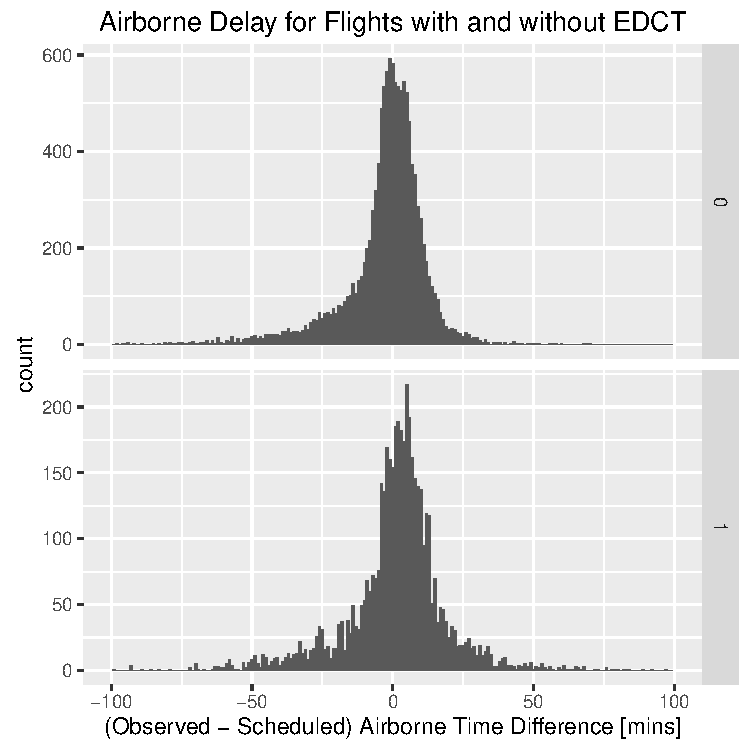
\includegraphics[scale=0.5]{abdiff_unw_faceted}
% where an .eps filename suffix will be assumed under latex, 
% and a .pdf suffix will be assumed for pdflatex; or what has been declared
% via \DeclareGraphicsExtensions.
\caption{Simulation results for the network.}
\label{fig_sim}
\end{figure}

% Note that the IEEE typically puts floats only at the top, even when this
% results in a large percentage of a column being occupied by floats.


% An example of a double column floating figure using two subfigures.
% (The subfig.sty package must be loaded for this to work.)
% The subfigure \label commands are set within each subfloat command,
% and the \label for the overall figure must come after \caption.
% \hfil is used as a separator to get equal spacing.
% Watch out that the combined width of all the subfigures on a 
% line do not exceed the text width or a line break will occur.
%
%\begin{figure*}[!t]
%\centering
%\subfloat[Case I]{\includegraphics[width=2.5in]{box}%
%\label{fig_first_case}}
%\hfil
%\subfloat[Case II]{\includegraphics[width=2.5in]{box}%
%\label{fig_second_case}}
%\caption{Simulation results for the network.}
%\label{fig_sim}
%\end{figure*}
%
% Note that often IEEE papers with subfigures do not employ subfigure
% captions (using the optional argument to \subfloat[]), but instead will
% reference/describe all of them (a), (b), etc., within the main caption.
% Be aware that for subfig.sty to generate the (a), (b), etc., subfigure
% labels, the optional argument to \subfloat must be present. If a
% subcaption is not desired, just leave its contents blank,
% e.g., \subfloat[].


% An example of a floating table. Note that, for IEEE style tables, the
% \caption command should come BEFORE the table and, given that table
% captions serve much like titles, are usually capitalized except for words
% such as a, an, and, as, at, but, by, for, in, nor, of, on, or, the, to
% and up, which are usually not capitalized unless they are the first or
% last word of the caption. Table text will default to \footnotesize as
% the IEEE normally uses this smaller font for tables.
% The \label must come after \caption as always.
%
%\begin{table}[!t]
%% increase table row spacing, adjust to taste
%\renewcommand{\arraystretch}{1.3}
% if using array.sty, it might be a good idea to tweak the value of
% \extrarowheight as needed to properly center the text within the cells
%\caption{An Example of a Table}
%\label{table_example}
%\centering
%% Some packages, such as MDW tools, offer better commands for making tables
%% than the plain LaTeX2e tabular which is used here.
%\begin{tabular}{|c||c|}
%\hline
%One & Two\\
%\hline
%Three & Four\\
%\hline
%\end{tabular}
%\end{table}


% Note that the IEEE does not put floats in the very first column
% - or typically anywhere on the first page for that matter. Also,
% in-text middle ("here") positioning is typically not used, but it
% is allowed and encouraged for Computer Society conferences (but
% not Computer Society journals). Most IEEE journals/conferences use
% top floats exclusively. 
% Note that, LaTeX2e, unlike IEEE journals/conferences, places
% footnotes above bottom floats. This can be corrected via the
% \fnbelowfloat command of the stfloats package.




\section{Conclusion}
The conclusion goes here.




% conference papers do not normally have an appendix


% use section* for acknowledgment
\section*{Acknowledgment}


The authors would like to thank...





% trigger a \newpage just before the given reference
% number - used to balance the columns on the last page
% adjust value as needed - may need to be readjusted if
% the document is modified later
%\IEEEtriggeratref{8}
% The "triggered" command can be changed if desired:
%\IEEEtriggercmd{\enlargethispage{-5in}}

% references section

% can use a bibliography generated by BibTeX as a .bbl file
% BibTeX documentation can be easily obtained at:
% http://mirror.ctan.org/biblio/bibtex/contrib/doc/
% The IEEEtran BibTeX style support page is at:
% http://www.michaelshell.org/tex/ieeetran/bibtex/
\bibliographystyle{IEEEtran}
% argument is your BibTeX string definitions and bibliography database(s)
\bibliography{IEEEabrv,/Users/ashah/NoBackup/code/nasa/src/causalInfFAA/doc/causalInfPaper/gdp_casual}
%
% <OR> manually copy in the resultant .bbl file
% set second argument of \begin to the number of references
% (used to reserve space for the reference number labels box)
%\begin{thebibliography}{1}
%
%\bibitem{IEEEhowto:kopka}
%H.~Kopka and P.~W. Daly, \emph{A Guide to \LaTeX}, 3rd~ed.\hskip 1em plus
%  0.5em minus 0.4em\relax Harlow, England: Addison-Wesley, 1999.
%
%\end{thebibliography}




% that's all folks
\end{document}


